\documentclass[14pt]{extbook}
\usepackage{multicol, enumerate, enumitem, hyperref, color, soul, setspace, parskip, fancyhdr} %General Packages
\usepackage{amssymb, amsthm, amsmath, latexsym, units, mathtools} %Math Packages
\everymath{\displaystyle} %All math in Display Style
% Packages with additional options
\usepackage[headsep=0.5cm,headheight=12pt, left=1 in,right= 1 in,top= 1 in,bottom= 1 in]{geometry}
\usepackage[usenames,dvipsnames]{xcolor}
\usepackage{dashrule}  % Package to use the command below to create lines between items
\newcommand{\litem}[1]{\item#1\hspace*{-1cm}\rule{\textwidth}{0.4pt}}
\pagestyle{fancy}
\lhead{Module4}
\chead{}
\rhead{Version A}
\lfoot{2958-5637}
\cfoot{}
\rfoot{test}
\begin{document}

\begin{enumerate}
\litem{
Graph the equation below.\[ f(x) = (x-4)^2 - 16 \]\begin{enumerate}[label=\Alph*.]
\begin{multicols}{2}\item 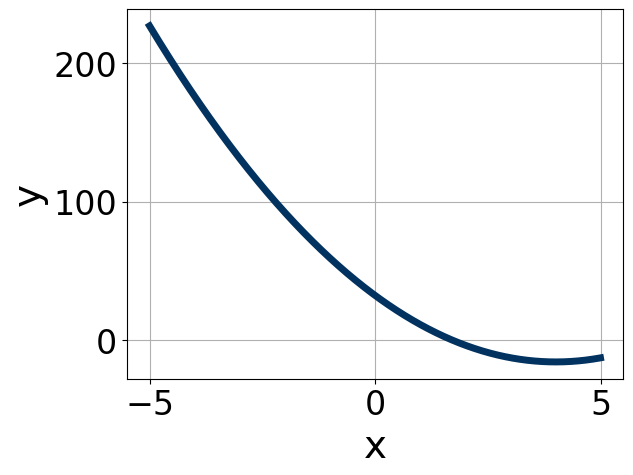
\includegraphics[width = 0.3\textwidth]{../Figures/quadraticEquationToGraphCopyAA.png}\item 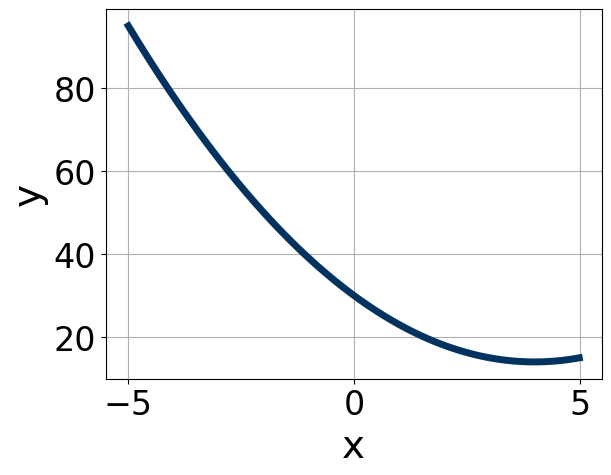
\includegraphics[width = 0.3\textwidth]{../Figures/quadraticEquationToGraphCopyBA.png}\item 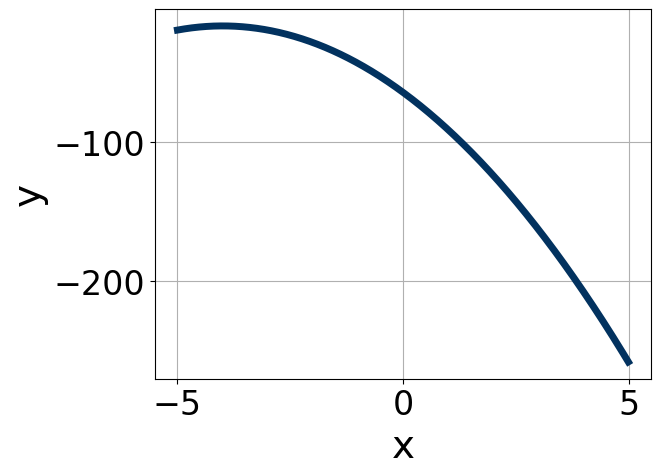
\includegraphics[width = 0.3\textwidth]{../Figures/quadraticEquationToGraphCopyCA.png}\item 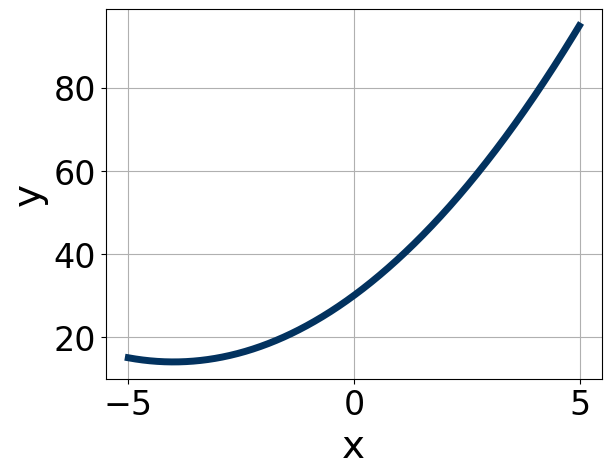
\includegraphics[width = 0.3\textwidth]{../Figures/quadraticEquationToGraphCopyDA.png}\end{multicols}\item None of the above.
\end{enumerate} }
\litem{
Factor the quadratic below. Then, choose the intervals that contain the constants in the form $(ax+b)(cx+d); b \leq d.$\[ 24x^{2} +50 x + 25 \]\begin{enumerate}[label=\Alph*.]
\item \( a \in [11.05, 12.72], \hspace*{5mm} b \in [2, 14], \hspace*{5mm} c \in [1.98, 2.67], \text{ and } \hspace*{5mm} d \in [3, 6] \)
\item \( a \in [2.45, 3.13], \hspace*{5mm} b \in [2, 14], \hspace*{5mm} c \in [7.5, 8.29], \text{ and } \hspace*{5mm} d \in [3, 6] \)
\item \( a \in [0.43, 1.83], \hspace*{5mm} b \in [19, 28], \hspace*{5mm} c \in [0.26, 1.26], \text{ and } \hspace*{5mm} d \in [30, 32] \)
\item \( a \in [4.46, 7.71], \hspace*{5mm} b \in [2, 14], \hspace*{5mm} c \in [3.96, 4.37], \text{ and } \hspace*{5mm} d \in [3, 6] \)
\item \( \text{None of the above.} \)

\end{enumerate} }
\litem{
Solve the quadratic equation below. Then, choose the intervals that the solutions belong to, with $x_1 \leq x_2$ (if they exist).\[ -13x^{2} -7 x + 7 = 0 \]\begin{enumerate}[label=\Alph*.]
\item \( x_1 \in [-21.31, -20.06] \text{ and } x_2 \in [19.89, 20.13] \)
\item \( x_1 \in [-1.26, -0.99] \text{ and } x_2 \in [-0.2, 0.73] \)
\item \( x_1 \in [-6.81, -6.12] \text{ and } x_2 \in [13.07, 13.86] \)
\item \( x_1 \in [-0.66, -0.16] \text{ and } x_2 \in [0.58, 1.16] \)
\item \( \text{There are no Real solutions.} \)

\end{enumerate} }
\litem{
Write the equation of the graph presented below in the form $f(x)=ax^2+bx+c$, assuming  $a=1$ or $a=-1$. Then, choose the intervals that $a, b,$ and $c$ belong to.
\begin{center}
    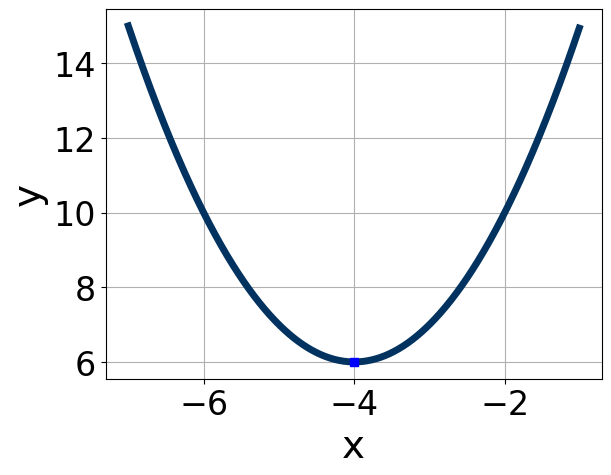
\includegraphics[width=0.5\textwidth]{../Figures/quadraticGraphToEquationA.png}
\end{center}
\begin{enumerate}[label=\Alph*.]
\item \( a \in [1, 5], \hspace*{5mm} b \in [-10, -3], \text{ and } \hspace*{5mm} c \in [7, 13] \)
\item \( a \in [-2, 0], \hspace*{5mm} b \in [-10, -3], \text{ and } \hspace*{5mm} c \in [-10, -8] \)
\item \( a \in [1, 5], \hspace*{5mm} b \in [6, 9], \text{ and } \hspace*{5mm} c \in [19, 24] \)
\item \( a \in [-2, 0], \hspace*{5mm} b \in [6, 9], \text{ and } \hspace*{5mm} c \in [-10, -8] \)
\item \( a \in [1, 5], \hspace*{5mm} b \in [-10, -3], \text{ and } \hspace*{5mm} c \in [19, 24] \)

\end{enumerate} }
\litem{
Solve the quadratic equation below. Then, choose the intervals that the solutions belong to, with $x_1 \leq x_2$ (if they exist).\[ -10x^{2} -13 x + 5 = 0 \]\begin{enumerate}[label=\Alph*.]
\item \( x_1 \in [-4.4, -2.8] \text{ and } x_2 \in [15.4, 16.9] \)
\item \( x_1 \in [-20.3, -19.3] \text{ and } x_2 \in [18.4, 19.6] \)
\item \( x_1 \in [-1.2, -0.1] \text{ and } x_2 \in [1.4, 2.9] \)
\item \( x_1 \in [-2.1, -0.6] \text{ and } x_2 \in [0, 1] \)
\item \( \text{There are no Real solutions.} \)

\end{enumerate} }
\litem{
Solve the quadratic equation below. Then, choose the intervals that the solutions $x_1$ and $x_2$ belong to, with $x_1 \leq x_2$.\[ 25x^{2} -10 x -24 = 0 \]\begin{enumerate}[label=\Alph*.]
\item \( x_1 \in [-0.52, -0.22] \text{ and } x_2 \in [1.92, 2.66] \)
\item \( x_1 \in [-1.68, -1.57] \text{ and } x_2 \in [0.27, 0.67] \)
\item \( x_1 \in [-20.14, -19.49] \text{ and } x_2 \in [29.9, 30.1] \)
\item \( x_1 \in [-1.1, -0.68] \text{ and } x_2 \in [0.61, 1.79] \)
\item \( x_1 \in [-4.51, -3.63] \text{ and } x_2 \in [0.05, 0.37] \)

\end{enumerate} }
\litem{
Solve the quadratic equation below. Then, choose the intervals that the solutions $x_1$ and $x_2$ belong to, with $x_1 \leq x_2$.\[ 25x^{2} -15 x -54 = 0 \]\begin{enumerate}[label=\Alph*.]
\item \( x_1 \in [-30.04, -29.15] \text{ and } x_2 \in [44.8, 45.08] \)
\item \( x_1 \in [-4.93, -3.14] \text{ and } x_2 \in [0.55, 0.7] \)
\item \( x_1 \in [-6.3, -4.62] \text{ and } x_2 \in [0.15, 0.51] \)
\item \( x_1 \in [-1.15, 0.07] \text{ and } x_2 \in [3.46, 3.65] \)
\item \( x_1 \in [-1.91, -1.14] \text{ and } x_2 \in [1.53, 2.08] \)

\end{enumerate} }
\litem{
Factor the quadratic below. Then, choose the intervals that contain the constants in the form $(ax+b)(cx+d); b \leq d.$\[ 54x^{2} +69 x + 20 \]\begin{enumerate}[label=\Alph*.]
\item \( a \in [26.3, 28.3], \hspace*{5mm} b \in [-1, 10], \hspace*{5mm} c \in [1.95, 2.38], \text{ and } \hspace*{5mm} d \in [5, 8] \)
\item \( a \in [2.7, 5], \hspace*{5mm} b \in [-1, 10], \hspace*{5mm} c \in [11.99, 12.1], \text{ and } \hspace*{5mm} d \in [5, 8] \)
\item \( a \in [0, 2.2], \hspace*{5mm} b \in [24, 26], \hspace*{5mm} c \in [0.91, 1.89], \text{ and } \hspace*{5mm} d \in [44, 50] \)
\item \( a \in [8.6, 10.1], \hspace*{5mm} b \in [-1, 10], \hspace*{5mm} c \in [5.85, 6.2], \text{ and } \hspace*{5mm} d \in [5, 8] \)
\item \( \text{None of the above.} \)

\end{enumerate} }
\litem{
Graph the equation below.\[ f(x) = -(x+3)^2 - 18 \]\begin{enumerate}[label=\Alph*.]
\begin{multicols}{2}\item 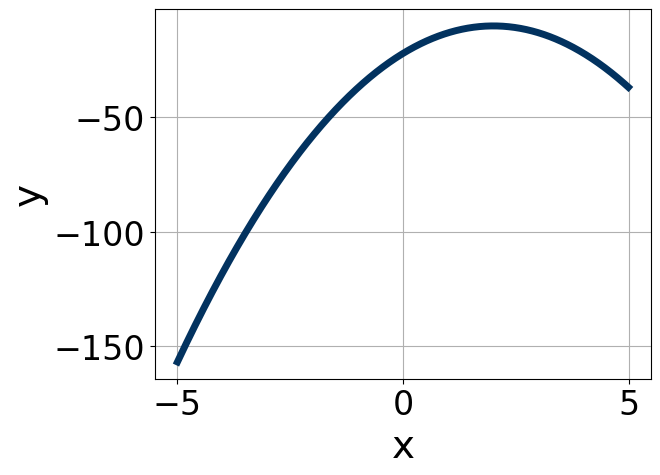
\includegraphics[width = 0.3\textwidth]{../Figures/quadraticEquationToGraphAA.png}\item 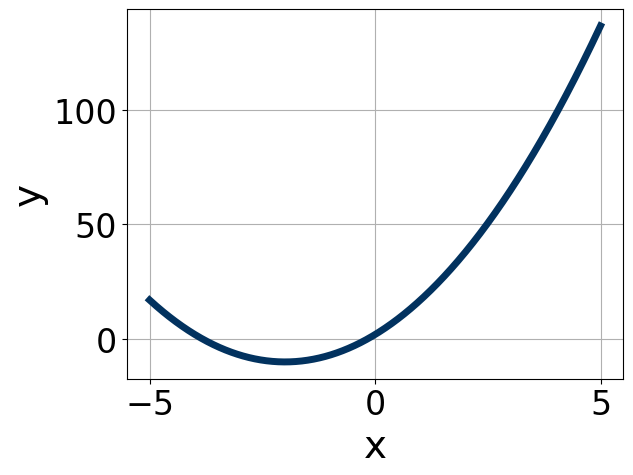
\includegraphics[width = 0.3\textwidth]{../Figures/quadraticEquationToGraphBA.png}\item 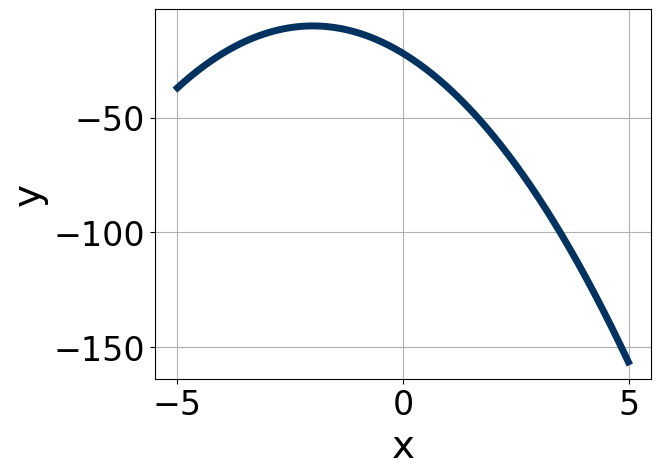
\includegraphics[width = 0.3\textwidth]{../Figures/quadraticEquationToGraphCA.png}\item 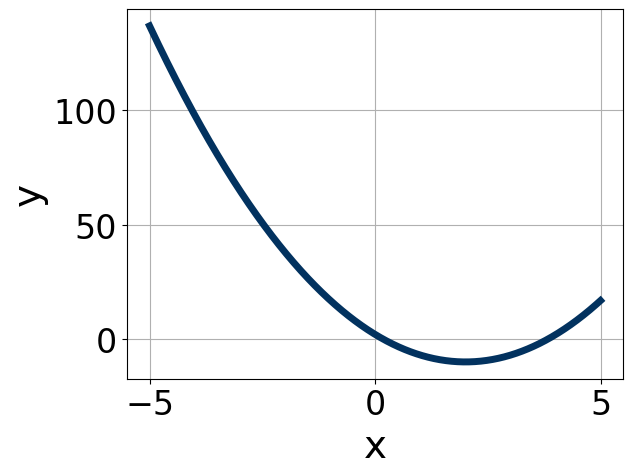
\includegraphics[width = 0.3\textwidth]{../Figures/quadraticEquationToGraphDA.png}\end{multicols}\item None of the above.
\end{enumerate} }
\litem{
Write the equation of the graph presented below in the form $f(x)=ax^2+bx+c$, assuming  $a=1$ or $a=-1$. Then, choose the intervals that $a, b,$ and $c$ belong to.
\begin{center}
    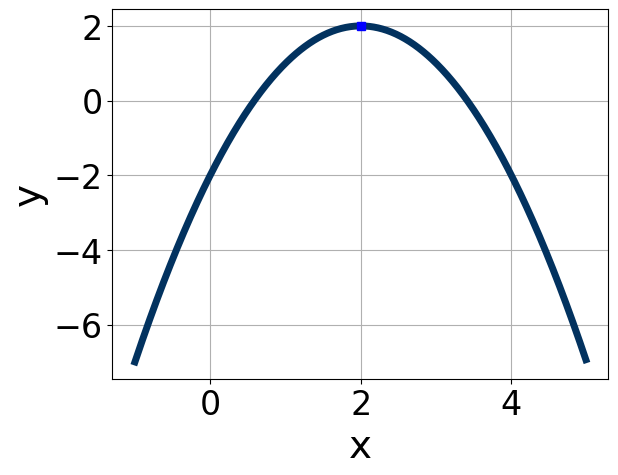
\includegraphics[width=0.5\textwidth]{../Figures/quadraticGraphToEquationCopyA.png}
\end{center}
\begin{enumerate}[label=\Alph*.]
\item \( a \in [-2.9, -0.5], \hspace*{5mm} b \in [3, 8], \text{ and } \hspace*{5mm} c \in [-11, -3] \)
\item \( a \in [0.9, 2], \hspace*{5mm} b \in [-5, -1], \text{ and } \hspace*{5mm} c \in [-2, 2] \)
\item \( a \in [0.9, 2], \hspace*{5mm} b \in [3, 8], \text{ and } \hspace*{5mm} c \in [-2, 2] \)
\item \( a \in [-2.9, -0.5], \hspace*{5mm} b \in [-5, -1], \text{ and } \hspace*{5mm} c \in [-11, -3] \)
\item \( a \in [-2.9, -0.5], \hspace*{5mm} b \in [-5, -1], \text{ and } \hspace*{5mm} c \in [-2, 2] \)

\end{enumerate} }
\end{enumerate}

\end{document}